\documentclass[a4paper,12pt]{article} %style de document
\usepackage[utf8]{inputenc} %encodage des caractères
\usepackage[french]{babel} %paquet de langue français
\usepackage[T1]{fontenc} %encodage de la police
\usepackage[top=2cm,bottom=2cm,left=2cm,right=2cm]{geometry} %marges
\usepackage{graphicx}
\usepackage{hyperref}
\usepackage{verbatim}
\usepackage{mathtools}
\usepackage{tikz}
\usepackage{tocbibind}
\usepackage{amsmath}
\usepackage{amsfonts}
\usepackage{amssymb}
\usepackage{fancyhdr}

\newcommand{\HRule}{\rule{\linewidth}{0.5mm}}

\setlength{\parskip}{\baselineskip}
\setlength{\headheight}{15pt} % Ajuste la hauteur de l'entête

\pagestyle{fancy}
\fancyhf{} % Nettoie tous les en-têtes et pieds de page
\fancyfoot[L]{
\includegraphics[width=1in]{logo.png}} % Logo à gauche en bas de chaque page
\rfoot{\textbf{Page \thepage}} % Numéro de page à droite
\renewcommand{\footrulewidth}{1pt} % Ligne de séparation au bas

\begin{document}
\begin{titlepage}
    \centering
    %% Contenu de la page de titre

    {\large Université de Caen Normandie}

    \begin{figure}[h]
        \centering
        
\includegraphics[width=0.4\textwidth]{logo.png}
    \end{figure}
    \vspace*{2cm}
    {\large Filière : Informatique\par}

    \vspace*{0.5cm}
    \HRule \\[0.4cm]
    {\huge \bfseries Intelligence Artificielle et Aide à la Décision \par}
    \HRule \\[0.4cm]

    \vspace*{\fill}

    % Author and supervisor
    \begin{minipage}{0.4\textwidth}
        \begin{center}
        	\textbf{Enseignant :}\\
        	 \textbf{M. BONNET Gregory}\\
        	  \textbf{Réalisé par :}\\
            \textbf{DIALLO Boubacar Sadio}\\
            \textbf{LAITH Alhazzaa}
        \end{center}
    \end{minipage}%
    \vspace*{\fill}
    
    \begin{figure}[h]
        \centering
        
\includegraphics[width=0.4\textwidth]{ia.jpg}
    \end{figure}
    
    {\large Fil Rouge Aide à la Décision et Intelligence Artificielle\\ Année Universitaire\\ 2024/2025}
\end{titlepage}

\tableofcontents
\newpage

\section{Introduction}
Le monde des blocs (\emph{BlocksWorld}) est un problème classique en intelligence artificielle, utilisé pour illustrer la planification et les problèmes de satisfaction de contraintes. Il se compose d'une série de blocs colorés pouvant être empilés les uns sur les autres pour former différentes configurations. L'objectif est souvent de déterminer une séquence d'actions permettant de transformer une configuration initiale en une configuration finale souhaitée.

Ce projet vise à modéliser un tel problème, explorer les algorithmes de planification et mettre en œuvre une solution logicielle utilisant des outils d'intelligence artificielle.

\section{Packages et Modules}
Les principaux modules développés et utilisés pour résoudre ce problème sont listés ci-dessous :

\begin{enumerate}
    \item \textbf{modelling :} Contient les classes et fonctions nécessaires pour modéliser le problème.
    \item \textbf{planning :} Gère les algorithmes de planification.
    \item \textbf{cp :} Représentation des contraintes pour la satisfaction de contraintes.
    \item \textbf{datamining :} Extraction de données pour l'analyse.
    \item \textbf{blocksworld :} Contient les sous-modules :
    \begin{enumerate}
        \item \textbf{block :} Représentation la structure de base et les fonctionnalités associées aux blocs.
        \item \textbf{executable :} Gère l'exécution.
    \end{enumerate}
\end{enumerate}

\section{Exemple d’un Monde des Blocs}
Voici un exemple de trois configurations possibles dans un monde des blocs :

\begin{figure}[h]
    \centering
    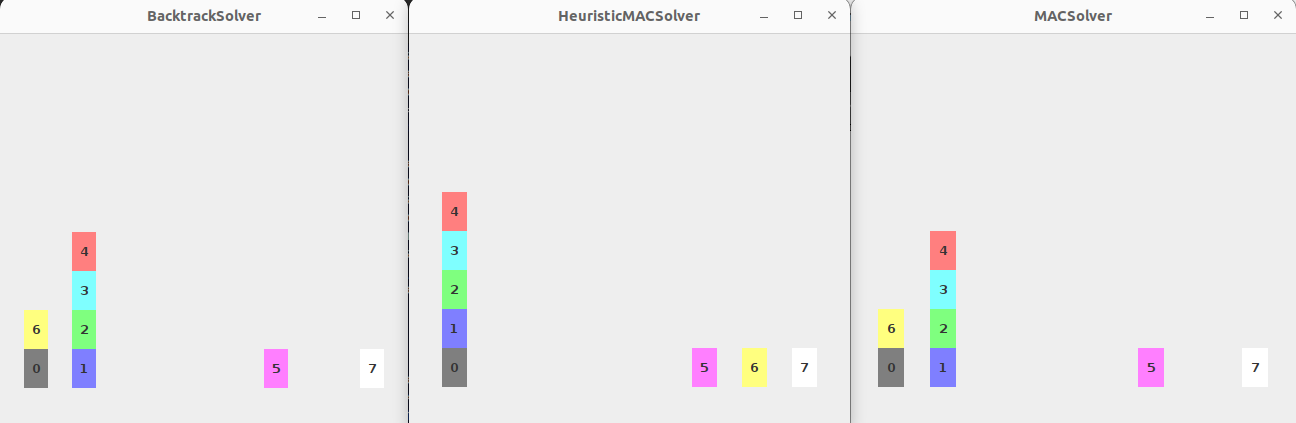
\includegraphics[width=0.8\textwidth]{ex.png}
    \caption{Trois configurations d’un monde des blocs.}
\end{figure}

\section{Diagramme de Classes de \emph{BlocksWorld}}
Le diagramme de classes suivant représente la structure de l'application pour le monde des blocs. Il met en évidence les relations entre les différents composants.

\begin{figure}[h]
    \centering
%    \includegraphics[width=0.8\textwidth]{dc.png} % Remplacez avec l'image du diagramme de classes.
    \caption{Diagramme de classes du projet \emph{BlocksWorld}.}
\end{figure}

\section{Planification dans \emph{BlocksWorld}}
La planification est au cœur du problème. Deux approches principales peuvent être utilisées :

\begin{enumerate}
    \item \textbf{Recherche de plan :} Utilisation d'algorithmes comme \emph{A*}, \emph{BFS} ou \emph{DFS}.
    \item \textbf{Satisfaction de contraintes :} Utilisation de solveurs pour déterminer la séquence optimale d'actions.
\end{enumerate}

Ces approches sont intégrées dans le module \texttt{planning} et sont testées pour évaluer leurs performances.

\section{Heuristiques pour le Monde des Blocs}
Pour résoudre efficacement le problème du monde des blocs, nous avons implémenté deux heuristiques admissibles. Ces heuristiques permettent d'estimer la distance entre un état courant et l'état final souhaité, facilitant ainsi la recherche d'un plan optimal à l'aide d'algorithmes comme \emph{A*}. 

\subsection{Présentation des Heuristiques}
\begin{enumerate}
    \item \textbf{Heuristique 1 : Vérification de la satisfaction du but}

    La première heuristique (\texttt{BlockWorldHeuristique1}) se concentre sur une approche simple : elle vérifie si l'état courant satisfait le but ou non. Si le but est satisfait, la valeur heuristique est 0. Dans le cas contraire, elle retourne 1. 

    Toutefois, cette heuristique n'est pas très informative, car elle ne distingue pas entre les différents états non terminaux.

    \item \textbf{Heuristique 2 : Comptage des blocs mal positionnés}

    La deuxième heuristique (\texttt{BlockWorldHeuristique2}) fournit une estimation plus précise en comptant le nombre de blocs qui ne sont pas dans leur position finale. Pour chaque bloc mal positionné, une valeur est ajoutée au compteur.
\end{enumerate}
Les deux heuristiques ont été soigneusement implémentées et testées dans le cadre de notre projet. Elles répondent aux critères suivants :
\begin{itemize}
    \item \textbf{Admissibilité :} Aucune des heuristiques ne surestime le coût réel pour atteindre l'objectif.
    \item \textbf{Utilité :} Dans nos tests avec des configurations variées du monde des blocs, elles ont permis de guider efficacement les algorithmes de recherche.
\end{itemize}

\section{Conclusion}
Le monde des blocs est un excellent outil pédagogique et pratique pour explorer les concepts de planification et de satisfaction de contraintes en intelligence artificielle. Ce projet vise à fournir une implémentation complète et modulable, adaptée aux besoins des chercheurs et étudiants.

L'implémentation est extensible, permettant d'ajouter des fonctionnalités supplémentaires comme des heuristiques avancées ou des visualisations interactives.

\vspace{2cm}
\begin{center}
    \textbf{Merci}
\end{center}

\end{document}
